\documentclass[twocolumn]{summery_4.1}

\title{Experimentalphysik IV - Zusammenfassung}

\begin{document}
\maketitle
\tableofcontents

\section{Erste Hinweise auf eine Diskretisierung auf der kleinsten Ebene}
\begin{itemize}
    \item \textbf{Gesetz der konstanten Proportionen:} In der Chemie wurde im 19. Jahrhundert entdeckt, dass viele chemische Reaktionen in ganzzahligen Verhältnissen ablaufen, z.B. für 100g Wasser: 11.1g Wasserstoff + 88.9g Sauerstoff $\to$ Massenverhältnis 1:8 
    \item \textbf{Gesetz konstanter Volumina:} Bei gleicher Temperatur und Druck reagieren Gase in konstanten ganzzahligen Volumenverhältnissen. Dies kann mit der idealen Gasgleichung so erklärt werden, dass bei gleicher Temperatur und Druck das  Volumenverhältnissen gleich dem Verhältnis an Teilchenzahlen ist $\frac{V_1}{V_2} = \frac{N_1}{N_2}$.
    \item\textbf{Periodizität chemischer Eigenschaften von Elementen mit Ordnungszahl $Z$:} Mitte des 19ten Jahrhunderts durch Dmitri Mendelejew und Lothar
    Meyer entdeckt; Führte zur Entwicklung des Periodensystems.
    \item\textbf{Brownsche Molekularbewegung:} Zitterbewegungen kleiner Mikropartikel aufgrund von zufälligen Kollisionen mit Atomen/Molekülen in der Umgebung.
\end{itemize}

\onecolumn
\section{Drehimpuls und magnetisches Moment}
\subsection{Drehimpuls}

\begin{description}
    \item[Beschreibung:] Eine klassisch verständliche Eigenschaft. 
    \item[Operator:] \(\v J = (J_x,J_y,J_z)\). Gehorcht der Vertauschungsrelation von Drehimpulsen \(\bug{J_x,J_y} = i\hbar J_z \). Da die drei Komponenten nicht mit einander vertauschen wählt man als maximal möglicher Satz vertauschbarer Operatoren \(\absv J\) und \(J_z\).
    
\begin{center}
    \begin{tabular}{lll}
        \toprule
        \multicolumn{3}{c}{\bf Bahndrehimpuls:}\\\midrule
        {\bf Größe} & {\bf Quantenzahl} & {\bf Wert}\\\midrule
        \(\v L \) &  & nicht scharf messbar \\
        \(\absv L\) & \(l=0,\dots, n-1\) & \(\sqrt{l(l+1)}\cdot \hbar \) \\
        \(L_z\) & \(m_l=0,\dots, \pm l \) & \(m_l \hbar \)\\\bottomrule
    \end{tabular}    
\end{center}

\item[Drehimpuls-Addition:]\,

{\bf Ausgangspunkt:} zwei Drehimpulse, mit v.S.k.O. und Eigenzuständen
\begin{align*}
    \v J_1^2,J_{1z},\v J_2,J_{2z} &\to \ket{j_1,m_1,j_2,m_2}
\end{align*}

Die beiden Drehimpulse koppeln zu einem Gesamtdrehimpuls \(\v J = \v J_1+\v J_2\).
Es gilt \(J_z = J_{1z}+J_{2z}\), aber die Basis besteht im allgemeinen nicht aus Eigenvektoren von \(\v J^2\).\\

{\bf Lösung:} Wechsel den v.S.k.O. zu
\begin{align*}
    \v J^2,J_z,\v J_1^1,\v J_2^2 &\to \ket{j,m,j_1,j_2}
\end{align*}
\vspace{-1ex}
\begin{center}
    \begin{tabular}{lll}
        \toprule
        \multicolumn{3}{c}{\bf Gesamtdrehimpuls:}\\\midrule
        {\bf Größe} & {\bf Quantenzahl} & {\bf Wert}\\\midrule
        {\(\v J = \v J_1 + \v J_2\)} & {} & {nicht scharf messbar} \\
        {\(\absv J\)} & {\(j=\abs{j_1-j_2},\dots,j_1+j_2\)} & {\(\sqrt{j(j+1)}\cdot \hbar \)} \\
        {\(J_z\)} & {\(m_j=m_{j_1}+m_{j_2}= -(j_1+j_2), \dots ,j_1+j_2 \)} & {\(m_j \hbar \) }\\\bottomrule
    \end{tabular}
\end{center}
\end{description}


\subsection{Spin}
\begin{description}
    \item[Beschreibung:] Rein quantenmechanische Eigenschaft, welche einem Drehimpuls ähneld. 
    \item[Operator:] \(\v S = (S_x,S_y,S_z)\). Gehorcht der Vertauschungsrelation von Drehimpulsen \(\bug{S_x,S_y} = i\hbar S_z \). Da die drei Komponenten nicht mit einander vertauschen wählt man als maximal möglicher Satz vertauschbarer Operatoren \(\absv S\) und \(S_z\).
    
    \begin{center}
        \begin{tabular}{@{}lll@{}}
            \toprule
            {\bf Größe} & {\bf Quantenzahl} & {\bf Wert}\\\midrule
            \(\v S\) & & nicht scharf messbar\\
            \(S_z\) & \(m_s\)  & \(S_z = m_s\hbar\)\\
            \(S\) & \(s=\frac12,1, \frac32,\dots \) & \(S = \sqrt{s(s+1)}\hbar\)\\\bottomrule
        \end{tabular}
    \end{center}

    \item[Verschiedene Teilchen:]\,\vspace{-1ex}
    
   \begin{center}
     \begin{tabular}{@{}lll@{}}
         \toprule
         {\bf Spin} & {\bf Typ} & {\bf Teilchen (Beispiele)}\\\midrule
         0 & Boson & Higgs-Boson \\
         \(\frac 12 \hbar\) & Fermion & Elektron, Proton, Neutrino, Quarks \\
         \(1\hbar\) & Boson & Photon, Gluon, W-Boson und Z-Boson \\\bottomrule
     \end{tabular}
   \end{center}\vspace{-1ex}
    Photonen mit \(m_s=+1\) sind rechts-zirkular polarisiert, \(m_s=-1\) sind links-zirkular polarisiert, linear polarisiertes Licht ist nicht etwa \(m_s=0\), sondern eine Überlagerung von zwei Photonen mit \(m_s=+1\) und \(m_s=-1\).
\end{description}

\subsection{Magnetisches Moment:}
\begin{description}
    \item[Beschreibung:] Magnetisches Moment das von einem Teilchen oder einem Verbund dieser ausgeht. Semiklassisch lässt sich das magnetische Moment auf die bewegten Ladungsträger z.B. in der Atomschale zurückführen. Demnoch führt jeder Drehimpuls eines Ladungsträgers zu einem B-Feld, jedoch ist auch die rein quantenmechanische Eigenschaft des Spins Ursache eines magnetischen Moments. Magnetisches Moment und Drehimpulse werden durch die gleichen Quantenzahlen beschrieben.
    
    \item[Operator:]\,\vspace{-1ex}
    
    \begin{center}
        \begin{tabular}{@{}lcc@{}}
            \toprule 
            {\bf Größe} & {\bf Quantenzahl} & {\bf Wert}\\\midrule
            \(\v \mu_J = (\mu_x,\mu_y,\mu_z)\) & & nicht scharf messbar\\
            \(\abs{\v \mu_J}\) & \(j\) & \(\abs{\v \mu_J} = -g_J \mu_B \sqrt{j(j+1)}\)\\
            \(\mu_z\) & \(m_j\)  & \(\mu_z = - g_J \mu_B m_j\)\\\bottomrule
        \end{tabular}
    \end{center}\vspace{1ex}

    \item[Lande-Faktoren:]\,\vspace{-1ex}
    \begin{center}
        \begin{tabular}{@{}lcc@{}}
            \toprule
            {\bf Bezug} & {\bf Formelzeichen} & {\bf Wert}\\\midrule
            Bahndrehimpuls & \(g_l\) & 1\\
            Spin & \(g_s\) & \(2.00232\)\\
            Wasserstoffatom (für \(\tug{\abs{\v \mu_J}}\))& \(g_J\) & \(1 + \frac{j(j+1) + m(m+1) - l(l+1)}{2 j(j+1)} \)\\
            Wasserstoff Atomkern & \(g_I=g_p\) & 5.6\\\bottomrule
        \end{tabular}
    \end{center}
\end{description}

\section{Erwartungswerte im Wasserstoff-Atom}
\begin{center}
    \tabbox{{\bf Physikalische Größe \(\mathbf{(n,l,m)}\)-Abhängigkeit}}
    {\begin{tabular}{l|c}
            Energie: & \(E_n = -\frac\Ry{n^2}\)  \\\hdashline
            Energiebeitrag durch B-Feld: & \(\Delta E_B = \mu_B m_l \absv B\)  \\\hdashline
            Radius: & \(\tug {r_{nl}} = \frac{a_0}{2} \hug{3n^2 - l(l+1)}
            \ge a_0 n^2\)\\\hdashline
            Periodendauer für Umlauf: & \(T_n \propto n^3\)\\\hdashline
            Strahlungslebensdauer: & \(\propto n^3\)\\\hdashline
            Krititsche Feldstärke: & \(E_c = \pi \varepsilon_0 \Ry^2 e^{-3} n^{-4}\)\\
    \end{tabular}}\label{tab:Erwartungswerte}\vspace{1cm}

    \begin{tabular}{@{}lll@{}}
        \toprule
        {\bf Physikalische Größe} & \multicolumn{2}{l}{\bf \(\mathbf{(n,l,m)}\)-Abhängigkeit}\\\midrule
        Energie & \(E_n\) & \(= -\frac\Ry{n^2}\)  \\
        Energiebeitrag durch B-Feld & \(\Delta E_B \) & \(= \mu_B m_l \absv B\)  \\
        Radius & \(\tug {r_{nl}} \) & \(= \frac{a_0}{2} \hug{3n^2 - l(l+1)}
        \ge a_0 n^2\)\\
        Periodendauer für Umlauf & \(T_n \) & \(\propto n^3\)\\
        Krititsche Feldstärke & \(E_c \) & \(= \pi \varepsilon_0 \Ry^2 e^{-3} n^{-4}\)\\\bottomrule
    \end{tabular}
\end{center}

\twocolumn

\section{Wasserstoff}
\subsection{Herleitung}
{\large DGL Gesamt}
\begin{align*}
    \hug{-\frac{\hbar^2}{2m_2} \Delta_e - \frac{\hbar^2}{2A m_p}\Delta_p + V(\v r_e, \v r_p)} \Psi(\v r_e, \v r_p) = E \,\Psi(\v r_e, \v r_p)
\end{align*}
mit 
\begin{align*}
    V(\v r_e, \v r_p) &= \frac{Z\, e^2}{4\pi \varepsilon_0 \abs{\v r_e - \v r_p}}
\end{align*}

Transformation ins Schwerpunkt und Relativsystem:
\begin{align*}
    \Psi(\v r, \v R) &= \psi(\v r)\cdot \varphi(\v R)
\end{align*}
mit 
\begin{align*}
    \v R = \frac{m_e \v r_e + A\, m_p \v r_p}{m_e + A \, m_p}&\tand \v r= \v r_e - \v r_p\\
    \v r_e = \v R + \frac{A\, m_p}{m_e + A\, m_p} &\tand \v r_p = \v R - \frac{m_e}{m_e + A\, m_p} \v r
\end{align*}

{\large Zerlegung der Gesamt-DGL}
{\bf DGL Schwerpunktbewegung}
\begin{align*}
    -\frac{\hbar^2}{2M} \Delta_R \varphi(\v R) &= E_s \varphi(\v R)\note M = m_e +A\cdot m_p
\end{align*}
\textit{Lösung:} Wellenpaket einer Teilchenwelle
\begin{align*}
    \varphi(\v R) &= \int\dk c(k) e^{i\v k \v R}
\end{align*}

{\bf DGL Relativbewegung}
\begin{align*}
    E_r \psi(\v r) &= -\frac{\hbar^2}{2\mu} \Delta_r \psi(\v r) + V(r) \psi(\v r) \\
    \mu &= \frac{Z m_e m_p}{m_e + Z m_p}\neq \frac1{1+\frac{m_e}{m_k}}
\end{align*}

\textbf{Zerlegung der Relativbewegung:}
\begin{align*}
    \psi(\v r) &= R(r) \cdot \Theta(\theta) \cdot \Phi(\phi)
\end{align*}

{\large DGL $\Phi(\phi)$}
\begin{align*}
    - \dd[2]{}\phi \Phi(\phi) &= m^2 \Phi(\phi)
\end{align*}
Randbedingungen:
\begin{align*}
    \Phi(\phi) &= \Phi(\phi+2\pi)\note 1 = \int_0^{2\pi} \Phi^* \Phi \dphi
\end{align*}
\textbf{Lösung:}
\begin{align*}
    \Phi(\phi) &= \frac{1}{\sqrt{2\pi}} e^{\pm i m \phi}\note m\in \Z 
\end{align*}
\textbf{Anmerkungen:}
\begin{align*}
    L_z \Phi(\phi) &= \hbar m\, \Phi(\phi)
\end{align*}

{\large DGL $\Theta(\theta)$}
\begin{align*}
    \hug{-\frac{1}{\sin\theta}\pp{}\theta \hug{\sin\theta\pp{}\theta}  + \frac{m^2}{\sin^2\theta}}\Theta(\theta) =  l(l+1)\Theta(\theta)
\end{align*}
Lösung:
\begin{align*}
    \Theta(\theta) &= (-1)^{\frac{m+\abs m}{2}} \sqrt{\frac{2l +1}{2} \frac{(l - \abs m)!}{(l+\abs m)!}} P_l^{\abs m}(\cos\theta) 
\end{align*}
mit \( P_l^{\abs m}(\cos\theta)\) als assoziierte Legendrepolynome, und \( l\in \N\te{ und } 0 \le \abs m \le l\).\\

\textbf{Anmerkungen:} \(\Upsilon_{l}^{(m)}=\Theta(\theta)\,\Phi(\phi) \equiv\) Kugelflächenfunktionen:
\begin{align*}
    \Upsilon_l^{(m)} &=  (-1)^{\frac{m+\abs m}{2}} \sqrt{\frac{2l +1}{2} \frac{(l - \abs m)!}{(l+\abs m)!}} P_l^{\abs m}(\cos\theta) e^{im\phi}
\end{align*}
\textbf{Eigenschaften:}
\begin{align*}
    \int_{\partial K} \d\Omega \hug{\Upsilon_{l'}^{(m')}}^* \Upsilon_{l}^{(m)} &= \delta_{l',l} \delta_{m',(m)} \\
    \sum_{m=-l}^l \sabs{\Upsilon_{l}^{(m)}}^2 &= \frac{2l + 1}{4\pi}
\end{align*}

{\large DGL $R(r)$}
\begin{align*}
    \hug{\pp{}r \hug{r^2\pp{}r} + \frac{2\mu r^2}{\hbar^2} \hug{E_r - V(r)}} R(r) = l(l+1) R(r)
\end{align*}
Nebenbedingung:
\begin{align*}
    R(\infty) =0
\end{align*}

\textbf{Lösung (Laguerre Polynome)}:
\begin{align*}
    R_{n,l}(r) &=  \sum_{j=1}^{n-1} b_j r^j e^{-\kappa r}
\end{align*}
mit 
\begin{align*}
    b_j &= 2b_{j-1} \frac{\kappa j - a}{j(j+1) - l (l+1)}\note j\ge l\\
    b_n &= 0\\ 
    \kappa &= \sqrt{\frac{-2\mu E_r}{\hbar^2}} \\
    a &= \frac{\mu Z e^2}{4\pi \varepsilon_0 \hbar^2} \equiv  \frac{Z}{a_0}\\
\end{align*}

Anmerkungen:
\begin{align*}
    E_r = -\frac{\mu Z^2 e^4}{32 \pi^2 \varepsilon_0^2 \hbar^2} \frac{1}{n^2} = - \frac{13.6\cdot Z^2}{n^2} \u{eV}
\end{align*}

\subsection{Kompakt} 
\begin{description}
    \item[Quantenzahlen:]
    Der Zustand eines Wasserstoff ähnlichen Atoms wird durch die fünf Quantenzahlen $(n,l,m_l,m_s)$ charakterisiert:
    \begin{itemize}
        \item {\bf Haubtquantenzahl:} \(
            n\in\N\)
        \item {\bf Drehimpuls-Quantenzahl:} \(\ell\in[0,\,n-1]\)
        mit der Buchstabenkonvention \((0,1,2,3,4,\dots)\equiv (s,p,d,f,g,\dots)\). 
        \item {\bf Magnetische Quantenzahl:} \(m\in[-\ell,\ell]\), mit der Buchstabenkonvention
        \((0,1,2,3,4,\dots)\equiv (\sigma, \pi, \delta, \varphi, \gamma,\dots )\).
        Diese Quantenzahl ist mit der Projektion des Drehimpuls verknüpft.
        \item {\bf Spin:} \(m_s = \pm \frac12\) mit der Notation \(\hug{\frac12, -\frac12}\equiv \hug{\uparrow, \downarrow}\), \(s = \frac12\) (für ein Elektron). 
        \item {\bf Gesamtdrehimpuls-Quantenzahl:} \(m_j = m_l + m_s\), \(j=\)
    \end{itemize} 

    \item[Notationen:]\,
    
        \begin{description}
            \item[{\normalfont Normal:}] \((n,l,m_l,m_s) \to nlm_lm_s\) mit den entsprechenden Buchstaben.
            \item[{\normalfont  Drehimpuls Notation:}] \((n,s,l,j)\to n^{2s+1}l_j\), nur \(l\) als Buchstabe sonst Zahlen
        \end{description}

    \item[Erwartungswerte:]\,
    
    Für ein wasserstoffähnliches Atom welches sich nicht in einem außerem Feld befindet, ist nur die Quantenzahl \(n\) relevant für die Energie. Damit ist die Entartung der Energieniveaus \(k= \sum_{\ell,m,m_s} =2n^2 \).  

    \item[Normaler Zeeman-Effekt:]
    Befindet sich das Wasserstoffatom in einem inhomogenen B-Feld, haben die Quantenzahlen \(l,m_l\) einen (kleinen) Beitrag zur Energie. Damit spalten sich die bekannten Energieniveaus weiter auf.     
    Es sind nur Übergänge erlaubt bei denen \(\Delta \ell=\pm 1\), entsprechend dem Spin eines Photons. Damit ist \(\Delta m = -1,0,1\).
    Anschaulich wird bei $\Delta m = \pm1$ die z-Komponente des Drehimpulses geändert
    und ein zirkular polarisiertes Photon erzeugt. Für den Fall $\Delta m = 0$ überlagern sich beide zirkulare
    Polarisationsrichtungen zu linear polarisiertem Licht.\\
    Die Auswahlregeln sind: \(\Delta s = 0, \Delta m_s=0, \Delta l =\pm 1, \Delta m_l = 0,\pm1\)

    \item[Anormaler Zeeman Effekt]
    Analog zum normalen Zeeman Effekt, jedoch berücksichtigt man nun auch das magnetische Moment, welches durch den Spin verursacht wird. 
    Also \(\v \mu \equiv \v \mu_J = \v \mu_l + \v \mu_s\). Außerdem geht man davon aus, dass das Magnetfeld so schwach ist, dass die Kopplung von \(\v L\) und \(\v S\) zu \(\v J\) nicht gestört wird. 
    \begin{align*}
        \Delta E &= - \tug{\v \mu_j}_z B = m_j g_j \mu_B B
    \end{align*}

    \item[Paschen-Back Effekt]
    Analog zum annormalen Zeeman Effekt, jedoch ist das Magnetfeld so stark, dass die Kopplung von \(\v L\) und \(\v S\) zu \(\v J\) gestört wird. 
    \begin{align*}
        \Delta E &= (g_l m_l + g_s m_s) \mu_B B 
    \end{align*}

    \item[Stark Effekt]
    Auch das Anlegen eines starken elektrischen Feldes \(\v {\mathcal E} = \mathcal E \cdot \v e_z  \) führt zu einer Aufspaltung der Energieniveaus. Die Ursache für die Verschiebung der Energienivaus ist, dass das Coulomb-Potenzial wie folgt modifiziert wird:
    \begin{align*}
        V=-\frac{e^2}{4\pi\epsilon_0} \frac1r + e\,\mathcal E \,z 
    \end{align*}
    Der radiale Abstand $r$ des Elektrons hängt von $l$ ab. Die Orientierung der Orbitale hängt von $m_l$ ab. Dadurch wird das Potential für das Elektron abhängig von $l$ und $m_l$ unterschiedlich modifiziert. Durch diesen Effekt wird die ursprüngliche Entartung von $l$ aufgehoben.Welche Aufspaltung wird nun erwartet?
    \begin{itemize}
        \item Der S-Zustand (\(l=0\)): Ist sphärisch symmetrisch. Es ist keine Aufspaltung erwartet.
        \item \(l\neq0\): Keine sphärische Symmetrie \(\to\) Aufspaltung mit \(\Delta E \propto \absv{{\mathcal E}}\) (linearer Stark-Effekt)
        \item \(l\neq 0\): Meist quadratischer Stark-Effekt. \(\Delta E =\propto \abs{\v{\mathcal E}}^2\). Ursache: E-Feld induziert ein permanentes elektrisches Dipol \(\v p_{el} = \alpha \v{\mathcal E}\). Dies führt zum zusätzlichen Term \(V_{el} = - \v p_{el} \v{\mathcal E}=-\alpha \abs{\v{\mathcal E}}^2\)
    \end{itemize}

    \item[Feinstruktur:]
    Verwendet man statt der Schrödingergleichung die relativistische Diracgleichung und nähert diese durch eine Reihenentwicklung, bekommt man in erster Ordnung drei weitere Terme zum nicht relativistischen Hamiltonoperator \(H_0\).
    \begin{align*}
        H &= H_0 + V_{ls} + V_{rel} + V_{D} \\
        V_{ls} &=  \frac{g_s \mu_B \mu_0 Z e}{8\pi m_e \hbar} \frac{1}{r^3} \v S \cdot \v L 
    \end{align*}
    Die Korrekturen sind: 
    \begin{description}
        \item[Spin-Bahn-Kopplung \(V_{ls}\):]
        Eine relativistische Betrachtung zeigt, dass sich durch den Bahndrehimpuls ein B-Feld im Elektron befindet, mit dem das magnetische Moment des Spins wechselwirken kann. Die neuen Energieniveaus sind:
        \begin{align*}
            E_{n,l,s} &= E_n - \v \mu_s\cdot\v B_l\\
            &= E_n \left(1- \frac{Z^2\alpha^2}{2n l\hug{l+\frac12}(l+1)}\cdot\right.
            \\&\qquad \left. \begin{cases}
                +l &\for j=l+\frac12\\
                -(l+1) &\for j=l-\frac12\\
            \end{cases}\right)
        \end{align*}
        \item[Relativistische Korrektur der kin. Energie \(V_{rel}\):]
        Relativistisch ist die kinetische Energie gegeben durch
        \begin{align*}
            E\sub{kin} &= m_0 c^2 \hug{\sqrt{1 + \frac{p^2 c^2}{m_0^2c^4}} - 1}\\
            \frac{p^2 c^2}{m_0^2c^4}\ll1 \to&\approx\frac{p^2}{2 m_0}-\frac{p^4}{8m_0^3 c^2}
        \end{align*}
        Damit ist der neue Hamiltonoperator
        \begin{align*}
            H &= \frac{p^2}{2m} + V - \frac{p^4}{8m_0^3 c^2}
        \end{align*}
        welcher über eine Störungsrechnung zu den neuen Energieniveaus 
        \begin{align*}
            E_{n,l} &= E_n \cdot\hug{1 - \frac{Z^2\alpha^2}{n}\hug{\frac{3}{4n} - \frac{1}{l+\frac12}}}
        \end{align*}
        führt.

        \item[Darwin-Term \(V_D\):] Relativistische Korrektur zur Potenziellen Energie. Die Darwinkorrektur betrifft nur \(l=0\) Zustände und ergibt sich quantitativ korrekt auch aus der Gleichung für die Energiekorrektur der LS-Kopplung, wenn man \(l=j-\frac12 =0\) einsetzt.
        \begin{align*}
            E_{n,js} = E_n\hug{1 - \frac{1}{2}\frac{Z^2\alpha^2}{n}}
        \end{align*}

        \item[Insgesamt:] Alle Korrekturen können zusammen addiert werden zu 
        \begin{align*}
            E_{n,j} &= E_n + \Delta E_{LS} + \Delta\sub{rel} + \Delta E\sub{Darwin}\\ 
            &= E_n \bug{1 + \frac{Z^2 \alpha^2}{n} \hug{\frac{1}{j + \half}}- \frac{3}{4n}}
        \end{align*}
    \end{description}


    \item[Hyperfeinstruktur:]
\end{description}



%%%%
\subsection{Korrekturen}

\subsubsection{Normaler Zeeman-Effekt:}
Befindet sich das Wasserstoffatom in einem inhomogenen B-Feld, haben die Quantenzahlen \(l,m_l\) einen (kleinen) Beitrag zur Energie. Damit spalten sich die bekannten Energieniveaus weiter auf.     
Es sind nur Übergänge erlaubt bei denen \(\Delta \ell=\pm 1\), entsprechend dem Spin eines Photons. Damit ist \(\Delta m = -1,0,1\).
Anschaulich wird bei $\Delta m = \pm1$ die z-Komponente des Drehimpulses geändert
und ein zirkular polarisiertes Photon erzeugt. Für den Fall $\Delta m = 0$ überlagern sich beide zirkulare
Polarisationsrichtungen zu linear polarisiertem Licht.\\
Die Auswahlregeln sind: \(\Delta s = 0, \Delta m_s=0, \Delta l =\pm 1, \Delta m_l = 0,\pm1\)

\subsubsection{Anormaler Zeeman Effekt}
Analog zum normalen Zeeman Effekt, jedoch berücksichtigt man nun auch das magnetische Moment, welches durch den Spin verursacht wird. 
Also \(\v \mu \equiv \v \mu_J = \v \mu_l + \v \mu_s\). Außerdem geht man davon aus, dass das Magnetfeld so schwach ist, dass die Kopplung von \(\v L\) und \(\v S\) zu \(\v J\) nicht gestört wird. 
\begin{align*}
    \Delta E &= - \tug{\v \mu_j}_z B = m_j g_j \mu_B B
\end{align*}

\subsubsection{Paschen-Back Effekt}
Analog zum annormalen Zeeman Effekt, jedoch ist das Magnetfeld so stark, dass die Kopplung von \(\v L\) und \(\v S\) zu \(\v J\) gestört wird. 
\begin{align*}
    \Delta E &= (g_l m_l + g_s m_s) \mu_B B 
\end{align*}

\subsubsection{Stark Effekt}
Auch das Anlegen eines starken elektrischen Feldes \(\v {\mathcal E} = \mathcal E \cdot \v e_z  \) führt zu einer Aufspaltung der Energieniveaus. Die Ursache für die Verschiebung der Energienivaus ist, dass das Coulomb-Potenzial wie folgt modifiziert wird:
\begin{align*}
    V=-\frac{e^2}{4\pi\epsilon_0} \frac1r + e\,\mathcal E \,z 
\end{align*}
Der radiale Abstand $r$ des Elektrons hängt von $l$ ab. Die Orientierung der Orbitale hängt von $m_l$ ab. Dadurch wird das Potential für das Elektron abhängig von $l$ und $m_l$ unterschiedlich modifiziert. Durch diesen Effekt wird die ursprüngliche Entartung von $l$ aufgehoben.Welche Aufspaltung wird nun erwartet?
\begin{itemize}
    \item Der S-Zustand (\(l=0\)): Ist sphärisch symmetrisch. Es ist keine Aufspaltung erwartet.
    \item \(l\neq0\): Keine sphärische Symmetrie \(\to\) Aufspaltung mit \(\Delta E \propto \absv{{\mathcal E}}\) (linearer Stark-Effekt)
    \item \(l\neq 0\): Meist quadratischer Stark-Effekt. \(\Delta E =\propto \abs{\v{\mathcal E}}^2\). Ursache: E-Feld induziert ein permanentes elektrisches Dipol \(\v p_{el} = \alpha \v{\mathcal E}\). Dies führt zum zusätzlichen Term \(V_{el} = - \v p_{el} \v{\mathcal E}=-\alpha \abs{\v{\mathcal E}}^2\)
\end{itemize}

\subsubsection{Feinstruktur:}
Verwendet man statt der Schrödingergleichung die relativistische Diracgleichung und nähert diese durch eine Reihenentwicklung, bekommt man in erster Ordnung drei weitere Terme zum nicht relativistischen Hamiltonoperator \(H_0\).
\begin{align*}
    H &= H_0 + V_{ls} + V_{rel} + V_{D} \\
    V_{ls} &=  \frac{g_s \mu_B \mu_0 Z e}{8\pi m_e \hbar} \frac{1}{r^3} \v S \cdot \v L 
\end{align*}
Die Korrekturen sind: 
\begin{description}
    \item[Spin-Bahn-Kopplung \(V_{ls}\):]
    Eine relativistische Betrachtung zeigt, dass sich durch den Bahndrehimpuls ein B-Feld im Elektron befindet, mit dem das magnetische Moment des Spins wechselwirken kann. Die neuen Energieniveaus sind:
    \begin{align*}
        E_{n,l,s} &= E_n - \v \mu_s\cdot\v B_l\\
        &= E_n \left(1- \frac{Z^2\alpha^2}{2n l\hug{l+\frac12}(l+1)}\cdot\right.
        \\&\qquad \left. \begin{cases}
            +l &\for j=l+\frac12\\
            -(l+1) &\for j=l-\frac12\\
        \end{cases}\right)
    \end{align*}
    \item[Relativistische Korrektur der kin. Energie \(V_{rel}\):]
    Relativistisch ist die kinetische Energie gegeben durch
    \begin{align*}
        E\sub{kin} &= m_0 c^2 \hug{\sqrt{1 + \frac{p^2 c^2}{m_0^2c^4}} - 1}\\
        \frac{p^2 c^2}{m_0^2c^4}\ll1 \to&\approx\frac{p^2}{2 m_0}-\frac{p^4}{8m_0^3 c^2}
    \end{align*}
    Damit ist der neue Hamiltonoperator
    \begin{align*}
        H &= \frac{p^2}{2m} + V - \frac{p^4}{8m_0^3 c^2}
    \end{align*}
    welcher über eine Störungsrechnung zu den neuen Energieniveaus 
    \begin{align*}
        E_{n,l} &= E_n \cdot\hug{1 - \frac{Z^2\alpha^2}{n}\hug{\frac{3}{4n} - \frac{1}{l+\frac12}}}
    \end{align*}
    führt.

    \item[Darwin-Term \(V_D\):] Relativistische Korrektur zur Potenziellen Energie. Die Darwinkorrektur betrifft nur \(l=0\) Zustände und ergibt sich quantitativ korrekt auch aus der Gleichung für die Energiekorrektur der LS-Kopplung, wenn man \(l=j-\frac12 =0\) einsetzt.
    \begin{align*}
        E_{n,js} = E_n\hug{1 - \frac{1}{2}\frac{Z^2\alpha^2}{n}}
    \end{align*}

    \item[Insgesamt:] Alle Korrekturen können zusammen addiert werden zu 
    \begin{align*}
        E_{n,j} &= E_n + \Delta E_{LS} + \Delta E\sub{rel} + \Delta E\sub{Darwin}\\ 
        &= E_n \bug{1 + \frac{Z^2 \alpha^2}{n} \hug{\frac{1}{j + \half}}- \frac{3}{4n}}
    \end{align*}
\end{description}

\subsubsection{Lamb-Shift}
Der Lamb-Shift Effekt ist eine Konsequenz daraus, dass das Quantenvakuum nicht leer ist, sondern über kurze Zeiträume hinweg virtuelle Partikel entstehen und vernichtet werden. 
Konkret:
\begin{enumerate}
    \item Um das Elektron rum entsteht ein \(e^+ e^-\) Paar. Dieses schirmt die wahre Elektronenladung ab, wie im Falle der Polarisation eines Dielektrikums. Damit wird die Coulomb Wechselwirkung leicht verändert.
    \item Durch die Emission und Absorption virtueller Teilchen führt das Elektron aus Gründen der Impulserhaltung eine Zitterbewegung auf einer radialen Bahn um die mittlere Bahn durch. 
    \begin{align*}
        \tug{E\sub{pot}} \propto \tug{\frac1{r}} \to \propto \tug{\frac{1}{r\pm\delta}}
    \end{align*}
    Die Änderung hängt von der radialen Form des Atomorbitals ab und damit von $n$ und $l$. Konsequenz ist die Aufhebung der \(l\)-Entartung bei gleichem \(j\). 
\end{enumerate}

\subsubsection{Hyperfeinstruktur:}
Die Hyperfeinstruktur ist analog zur Feinstruktur, nur dreht es sich um die Kopplung dea Kernspins \(\v I\) mit dem Gesamtdrehimpuls der Hülle \(\v J\) zu dem Gesamtdrehimpuls \(\v F = \v I + \v J \).
Der Beitrag der Hyperfeinstruktur zu den Energieniveaus ist 
\begin{align*}
    \Delta E_{HFS} &= \frac A2 \hug{F(F+1) - j(j+1) - I(I+1)} \\
    A&=\frac{g_i \mu_K B_j}{\sqrt{j(j+1)}}
\end{align*}

Für zwei aufeinanderfolgende Energieniveau gilt:
\begin{align*}
    \Delta E_f &= \Delta E_{HFS,f+1}- \Delta E_{HFS,f} =  A\cdot (f+1)
\end{align*}
%%%%

\section{Viel Elektron Atome}
\subsection{Abschirmung}
Die Elektronen werden in Mehrelektronenatomen abhängig vom Energiezustand unterschiedlich stark abgeschirmt. Allgemein muss für die Energie gelten:
\begin{align*}
    \underbrace{-\frac{Z e^2}{4\pi \varepsilon_0 r}}\sub{Kernähe}\le V(r)\le \underbrace{-\frac{e^2}{4\pi \varepsilon_0 r}}\sub{außen}
\end{align*} 

\subsection{Polarisation}
Nicht nur abhängig von $n$ sondern auch von $l$ wird die äußere Hülle der Rumpfelektronen abhängig von dem Anregungszustand unterschiedlich polarisiert. Somit sind auch die Energieniveaus
von $n$ und $l$ abhängig. Dies wird durch einen Korrekturfaktor1 beschrieben:
\begin{align*}
    E_n\propto \frac{1}{n^2}\to E_{n,l} \propto \frac{1}{n^2\hug{1-\frac{\delta_{n,l}}{n}}^2}
\end{align*}

\subsection{Drehimpuls-Kopplungen}
Im allgemeinen sehr kompliziert, daher nur zwei Extremfällte.
\begin{description}
    \item[LS-Kopplung] 
    \begin{description}
        \item[Wann?] Diese Kopplung tritt auf wenn die magnetische Wechselwirkung zwischen den Spins der Elektronen
        und zwischen den Bahndrehimpulsen der Elektronen stärker ist, als die Wechselwirkung zwischen dem
        Spin und Bahndrehimpuls für jedes Elektron separat.
        \item[Kopplung:]
        Es koppeln sich erst alle Spins sowie Bahndrehimpuls zu einem gesamt Spin und Bahndrehimpuls:
        \begin{align*}
            \v S &= \sum_i \v s_i \tand \v L =\sum_i \v l_i 
        \end{align*} 
        \item[Quantenzahlen:] \(S,L,m_S, m_L \)
        \begin{align*}
            \abs{\v L} &= \sqrt{L(L+1)}\hbar\\
            \abs{\v S} &= \sqrt{S(S+1)}\hbar
        \end{align*} 
        \item[Aufspaltung:]
        \item[] \begin{align*}
            E &= E_{n,L,S} + C \,\v L \cdot \v S \note C\propto \frac{Z^4}{n^3}
        \end{align*}
    \end{description}
    \item[$jj$-Kopplung]
    \begin{description}
        \item[Wann?] Diese Kopplung tritt auf wenn die magnetische Wechselwirkung zwischen jedem Spin und seinem
        Bahndrehimpuls stärker ist als die Wechselwirkungen zwischen den Spins und zwischen den Bahndrehimpulsen. Diese Kopplung tritt eher bei schweren Atomen auf. 
        \item[Kopplung:]
        Es koppeln sich erst Bahndrehimpuls und Spin für jedes Elektron.
        \begin{align*}
            \v j_i &= \v l_i + \v s_i \tand \v J = \sum_i \v j_i 
        \end{align*} 
        \item[Quantenzahlen:] \(S,L,m_S, m_L \)
        \begin{align*}
            \sabs{\v L} &= \sqrt{L(L+1)}\hbar\\
            \sabs{\v S} &= \sqrt{S(S+1)}\hbar
        \end{align*} 
        \item[Aufspaltung:]
        \item[] \begin{align*}
            E &= E_{n,L,S} + C \,\v L \cdot \v S \note C\propto \frac{Z^4}{n^3}
        \end{align*}
    \end{description} 
    \item[Intermedäre Kopplung]
    Eine Mischung aus LS-/ und \(jj\)-Kopplung. Typischerweise die Realtität.
\end{description}

\subsection{Besetzungsregel}

\section{Atomübergänge und Strahlung}
\subsection{Kategorisierung}
Die möglichen Übergange von Atomen können in vier Kategorien verteilt werden:
\begin{description}
    \item[Absorption:] Befindet sich ein Atom des Zustandes $E_k$ in einem Strahlungsfeld, können Photonen absorbiert
    werden, die der Energiedifferenz zu einem angeregten Zustand $E_j$ entsprechen. Die Wahrscheinlichkeit für diesen Vorgang ist:
    \begin{align*}
        W_{k\to j} = B_{kj}\cdot u_\nu (\nu)
    \end{align*}
    mit \(B_{kj}\) als Einstein-Koeffizient für die Absorption (Reziprokwert der $1/e$-Zerfallszeit) und \(u_\nu(\nu)=h\nu\cdot n_\nu= h\nu \cdot \dd n\nu \) als spektrale Photonendichte des Strahlungsfeldes, d.h. Photonen pro Frequenz und Volumen. 
    \item[Spontane Emission:] Befindet sich ein Atom in einem angeregten Zustandes $E_j$, kann es spontan unter Aussendung von Licht in einen Zustand niedrigerer Energie übergehen. Die Wahrscheinlichkeit für diesen Vorgang ist:
    \begin{align*}
        W_{j\to k}^{\te{spontan}} = A_{j\to k}    
    \end{align*} mit \(A_{j\to k }\) als Einstein-Koeffizienten.
    \item[Induzierte Emission:] Trifft Licht auf ein Atom im angeregten Zustand $E_j$ kann der Übergang in ein tieferes Niveau $E_k$ angeregt werden. Wie Wahrscheinlichkeit ist:
    \begin{align*}
            W_{j\to k }^\te{ind} &= u_\nu (\nu) \cdot B_{j\to k }
    \end{align*}
    \item[Strahlungsloser Übergang:] Durch Stöße können auch verbotene Übergänge strahlungslos und damit unsichtbar induziert
    werden. Die Wahrscheinlichkeit \(R_i\) für diesen Vorgang hängt von der Temperatur und der Teilchendichte \(n\) ab.
    \begin{align*}
        R_i \propto n \,v\sub{rel}(T)\propto \frac{p}{\sqrt T}
    \end{align*}
\end{description}

\subsection{Berechnung der Einsteinkoeffizienten}
Durch Betrachtung des Erwartungswertes des Dipoloperators \(\tug{\v p\sub{el}}\) ergibt sich: 
\begin{align*}
    A_{kj} &= \frac{P}{\hbar \omega_{kj}}=\frac23 \frac{\omega_{kj}^3}{\epsilon_0 c^3 h}\abs{M_{kj}}^2\\
    B_{kj} &= \frac{1}{6\hbar^2 \epsilon_0} \abs{M_{kj}}^2 
\end{align*}
mit dem Matrixelement \(M_{kj}\) des Dipoloperators als 
\begin{align*}
    M_{kj} = \bra{\psi_k} q\v r \ket{\psi_j}
\end{align*}

Zwischen den Einsteinkoeffizienten gilt der folgenden Zusammenhang:
\begin{align*}
    B_{kj} &= \frac{c^3} {8\pi h \nu^3}A_{kj} =\frac{g_j}{g_k} B_{jk}
\end{align*}
mit \(g_j\) als Entwartung der Energiezustände

\subsection{Messung der Einsteinkoeffizienten}
Die Lebensdauer \(\tau_i\) eines Zustandes \(E_i\) ist gegeben durch
\begin{align*}
    \frac{1}{\tau_i} &= A_i + R_i= \sum_j \hug{A_{ij} + R_{ij}}
\end{align*}
Misst man zusätzlich die relativen Linienintensitäten \(I_{ij}\), können die einzelnen \(A_{ij}\) bestimmt werden als (mit \(R_i = 0\))
\begin{align*}
    A_{ik} = A_i \cdot \frac{\frac{I_{ik}}{h\nu_{ik}}}{\sum_j \frac{I_{ij}}{h\nu_{ij}}}
\end{align*}

\subsection{Elektrische Multipolstrahlung}
Es gibt auch Übergange die anderen Ordungen der elektrischen Multipolentwicklung entsprechen.
Für den Quadrupol ergibt sich z.B. Auswahlregen \(\Delta l=0,\pm2\), d.h. es werden zwei Photonen emittiert.

\subsection{Breite von Spektrallinien}
\begin{description}
    \item[Heisenberg'sche Unschärferelation:]
    Die Heisenberg'sche Unschärferelation gibt basierend auf der Lebensdauer \(\tau\) eines Zustandes eine untere Schranke für die Breite der Linie:
    \begin{align*}
        \Delta \nu &\ge \frac{1}{4\pi \tau}\\
        \Delta \lambda &\ge \frac{\lambda^2}{4\pi c \tau }
    \end{align*} 
    \item[Form der Spektrallinie:]
    Der Ansatz einer exponentiell abfallenden Strahlungsleistung führt zu einem Frequenzspektrum mit Lorentzprofil, bzw. Cauchyverteilung in der Wahrscheinlichkeitsrechnung.
    \begin{align*}
        P(\omega) &= P_0 \frac{\gamma/2}{(\omega-\omega_0)^2 + (\gamma/2)^2} 
    \end{align*}
    Die Halbwertsbreite entspricht dem Einsteinkoeffizient des Übergangs.
    \begin{align*}
        \delta_\omega = 2\pi \delta_f = A_i = \frac1\tau
    \end{align*}
    \item[Druckverbreiterung:]
    Durch die Wechselwirkung der Atomhüllen treten leichte Änderungen der Energieniveaus auf. Hierdurch werden Spektrallinien um $\Delta \nu$ verschoben. Außerdem verkürzt sich die Lebensdauer der Zustände durch von Kollisionen verursachte Übergange. Dadurch wird die Linie breiter. (Anwendung: Messung der Größe von Sternen)
    \item[Dopplerverbreiterung:]
    Atome in einem heißen Gas bewegen sich relativ zum Beobachter, deshalb kann der Dopplereffekt relevant werden.
    \begin{align*}
        \frac{\omega}{\omega_0} &= \sqrt{\frac{1-\beta}{1+\beta}}
        \overset{v\ll c}\approx 1-\beta 
    \end{align*}
    Die Geschwindigkeitesverteilung in radialer Richtung folgt einer Maxwellverteilung, sodass die Linienverbreiterung Gaußförmig wird.
    Die Breite wächst mit \(\sqrt T\) an:
    \begin{align*}
        \delta \lambda\sub{Doppler} 
    &= 2\sqrt{2\ln 2 }\cdot \Delta\lambda\sub{Doppler}\\
    \Delta \lambda\sub{Doppler}&= \frac{\lambda}{c} \sqrt{\frac{k_B T}{m}}\\
    \Delta f\sub{Doppler}&= \sqrt{\frac{k_B T}{mc^2}} f\\
    \end{align*}
\end{description}

\subsection{Röntgenstrahlung}
\begin{description}
    \item[Streuung und Absorbtion:] Jedes Photon hat eine konstante Wahrscheinlichkeit pro Zeiteinheit gestreut oder absorbiert zu werden, daher gilt für die Strahlungsleistung \(P\) nach der Absorberdicke \(x\) das Exponentialgesetzt
    \begin{align*}
        P(x) &= P_0 e^{-\mu x}, \mu = \sigma n
    \end{align*}  
    mit $\mu = \mu_s+\alpha$, \(\mu_s\) als Streukoeffizient und \(\alpha\) als Absorptionskoeffizient.
    \item[Streuung:] Hier gibt es drei wesendliche Streuprozesse ($E_B$ Bindungsenergie des Elektrons):
    \begin{description}
        \item[Rayleigh Streung] \(h\nu  \le E_B\). Es werden in den Atomhüllen elektrische Dipole angeregt.   
        \item[Thomson-Streuung] \(E_B\ll h\nu\ll m_ec^2\). Der Rückstoß des Elektrons ist vernachlässigbar, und das Photon wird mit gleicher Frequenz gestreut 
        \item[Comptonstrahlung] \(E_B\ll h\nu \approx m_ec^2\). Rückstoß ist nicht vernachlässigbar und es kommt zur Frequenzänderung beim Photon.  
    \end{description}
    \item[Absorbtion:] Für die Absorbtion bei höheren Energien sind im wesendlichen zwei Effekte relevant:
    \begin{description}
        \item[Photoeffekt] \(h\nu + A\to A^+ + e-\). Maximal Wahrscheinlichkeit für \(h\nu \approx E_B\), außerdem \(\alpha\propto Z^{4.5}\).
        \item[Paarbildung] \(h\nu + A \to A + e^+ + e^-\). Minimale Energie \(2 m_e c^2 \approx 1022\u{keV}\), und \(\alpha\propto Z^2\) 
    \end{description}
    \item[Wirkungsquerschnitt:] \(R = \sigma\cdot \Phi_\gamma \cdot N\sub{Target}\), \(R\) Reaktionsrate,\(\sigma, [\sigma]=m^2\) Proportionalitätskonstante, \(\Phi_\gamma\) Photonenfluss, \(N\sub{Target}\) Anzahl der Target-Teilchen. Es gilt \(\mu = \sigma n =\sigma \cdot \rho \frac{N_A}A\), \(n\) Menge an Target-Teilchen. 
    \item[Massenabschwächungskoeffizient:] \(\kappa =\frac{\mu}\rho\)
\end{description}
\subsubsection{Bremsstrahlung}


\section{Laser}
\subsection{Grundlagen}
Laser steht für {\bf \large L}aser {\bf\large A}mplification by {\bf\large S}timulated {\bf\large E}mission of {\bf\large R}adiation.\\[1ex]
Grundlage des Laser-Effekts ist die \emph{stimulierte Emission} von Photonen aus einem angeregten Zustand. \\
Hierbei wird durch ein einlaufendes Photon der richtigen Frequenz ein kohärenter Übergang angeregt und dabei ein Photon mit: 
1) \emph{gleicher Frequenz}, 2) \emph{Polarisation}, 3) \emph{Ausbreitungsrichtung} und 4)
\emph{fester Phasenbeziehung} erzeugt. Es kommt somit zur Lichtverstärkung.
Zusätzlich zur stimulierten Emission existieren zwei weitere konkurrierende Prozesse, die nicht zur Lichtverstärkung führen: Die spontane Emission und die Absorption aus dem Grundzustand.\\[1ex]

\subsubsection{Besetzungsinversion}
Damit es zu einer Lichtverstärkung kommen kann, benötigt man ein aktives Medium, d.h. es liegt eine Besetzungsinversion vor in dem mehr Teilchen im angeregten Niveau sind, als im Grundzustand. Die Inversionsbedingung ist 
\begin{align*}
    N_2 \gg N_1 \frac{g_2}{g_1}
\end{align*}
mit \(N_{1,2}\) als Teilchenzahl im Energieniveau und \(g_{1,2}\) als Entartung der Niveaus.

\subsubsection{Drei Niveau System}
\begin{description}
    \item[Grundzustand \(E_1\):] Aus diesem Niveau werden mitteln optischen Pumpens Zustände aus dem Energieniveau \(E_3\) angeregt.
    \item[Metastabiler Zustand \(E_3\):] Dieser Zustand ist metastabil, d.h. er kann aufgrund der Auswahlregeln nicht direkt in den Grundzustand verfallen. Der Zustand zerfällt schnell in den Zustand \(E_2\), verglichen mit der Zerfallzeit von \(E_2\to E_1\). So kann eine Inversion von \(E_1\) bezüglich 
    \(E_2\) erzeugt werden.
    \item[Angeregter Zustand \(E_2\):] Dieser zerfällt mit Strahlung in \(E_1\) ist ist die eigentliche Quelle des Laserlichts.   
\end{description}
\begin{figure}[H]
    \centering
    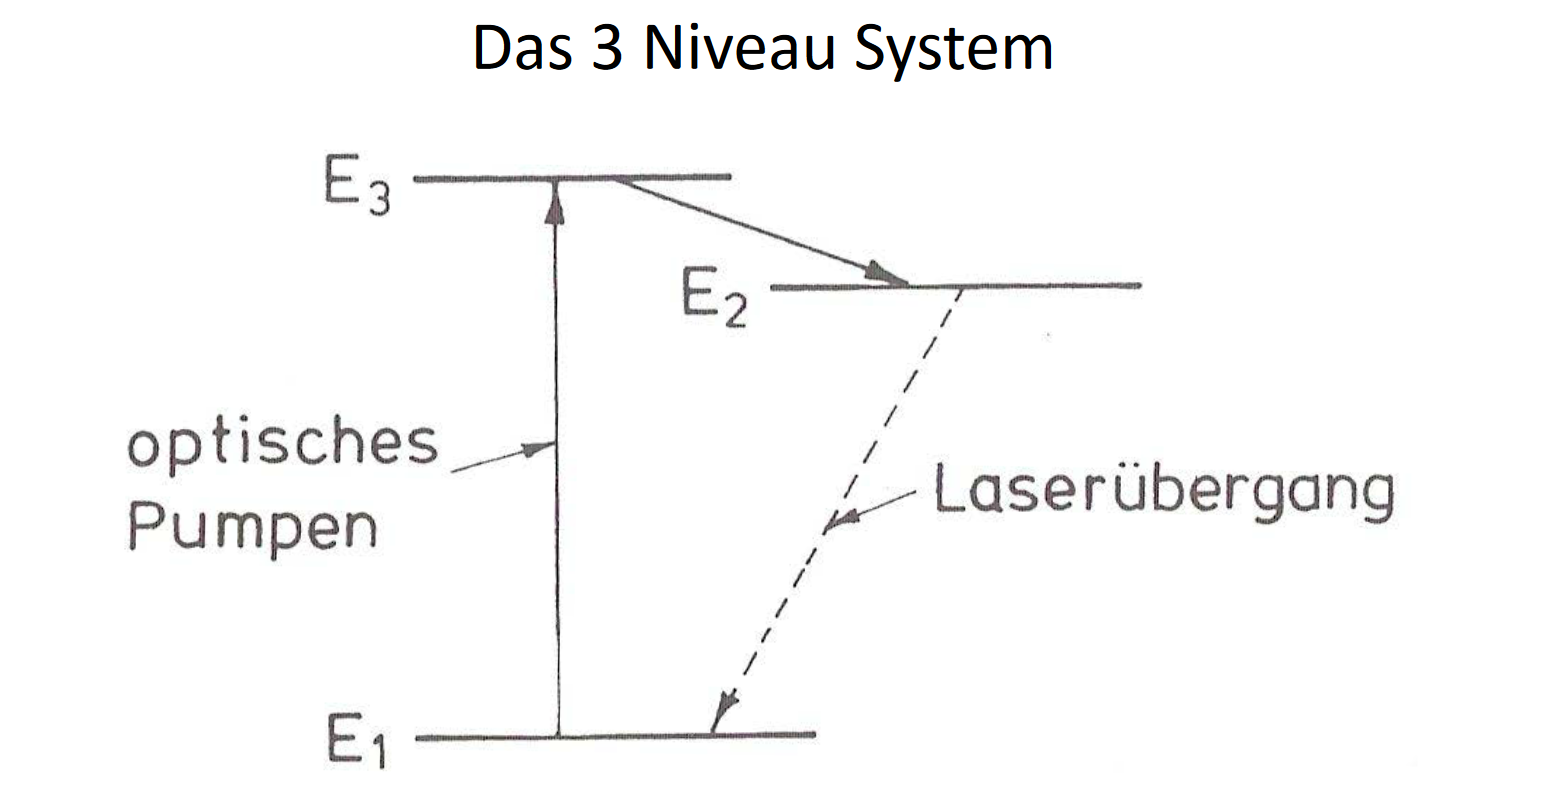
\includegraphics[width=.49\textwidth]{3_Niveau_Laser.png}
\end{figure}

\subsubsection{Resonator}
Problem: Der mit der induzierten Emission konkurrierende Prozess der spontanen Emission steigt mit zunehmender Frequenz, da dieser antiproportional ist zur Photonendichte aber proportional zur Modenzahldichte.\\

Lösung: Die spontane Emission kann entweder durch eine hohe Photonendichte unterdrückt werden, oder indem man die Modenzahldichte mit einem Resonator einschränkt. Moden, die die Resonanzbedingung \(m\cdot \lambda/2 = n L\note m\in\N \) erfüllen sind dann sehr stark besetzt.

\begin{figure}[H]
    \centering
    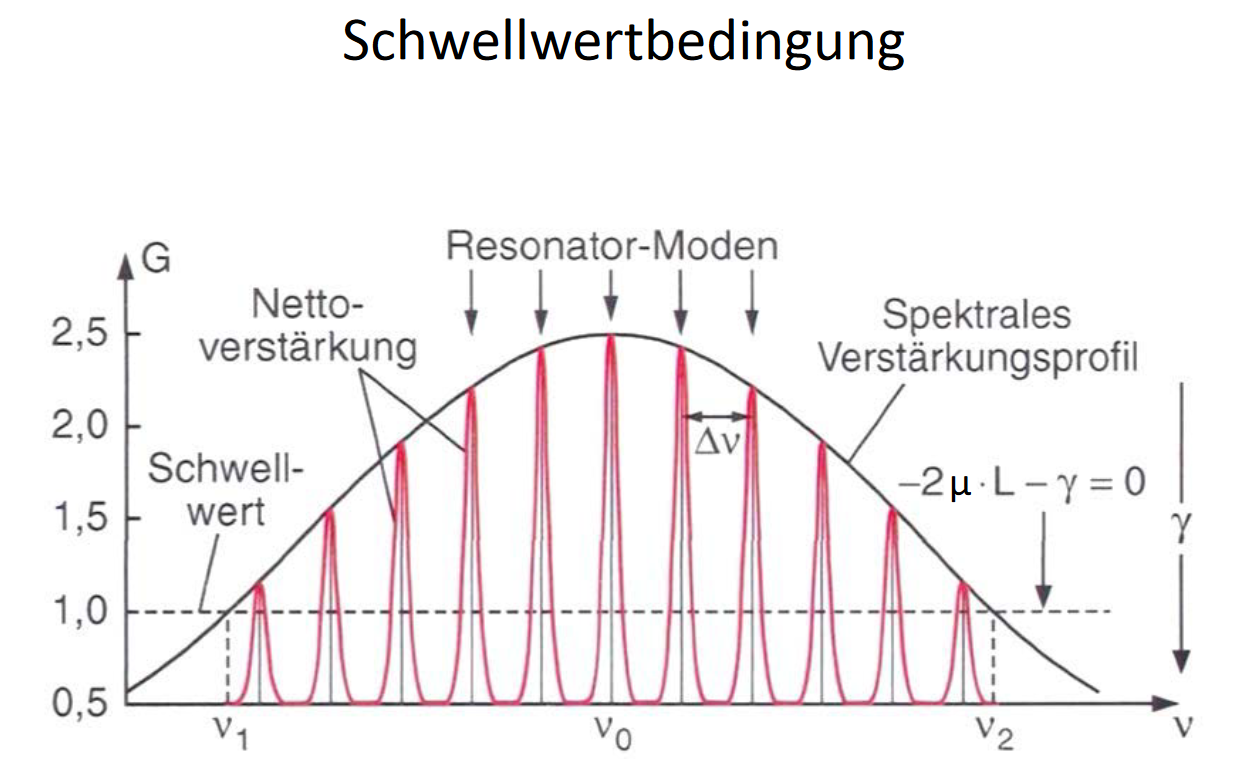
\includegraphics[width=.49\textwidth]{Schwellwertbedingung.png}
\end{figure}

Für eine Verstärkung muss die \emph{Schwellwertbedingung} erfüllt sein 
\begin{align*}
    -2\mu \cdot L > \gamma 
\end{align*}
mit Resonatorlänge \(L\), Wahrscheinlichkeit eines Photonenverlustes \(\gamma\) und der effektiven Abschwächung \(\mu = \mu\sub{abs}+\mu\sub{ind}\)
\(= \underbrace{\hug{n_k - \frac{g_k}{g_j}n_j}}\sub{Besetzungsinversion}\cdot \sigma(\nu)\), \(I(z)\propto e^{-\mu z}\).

\begin{figure}[H]
    \centering
    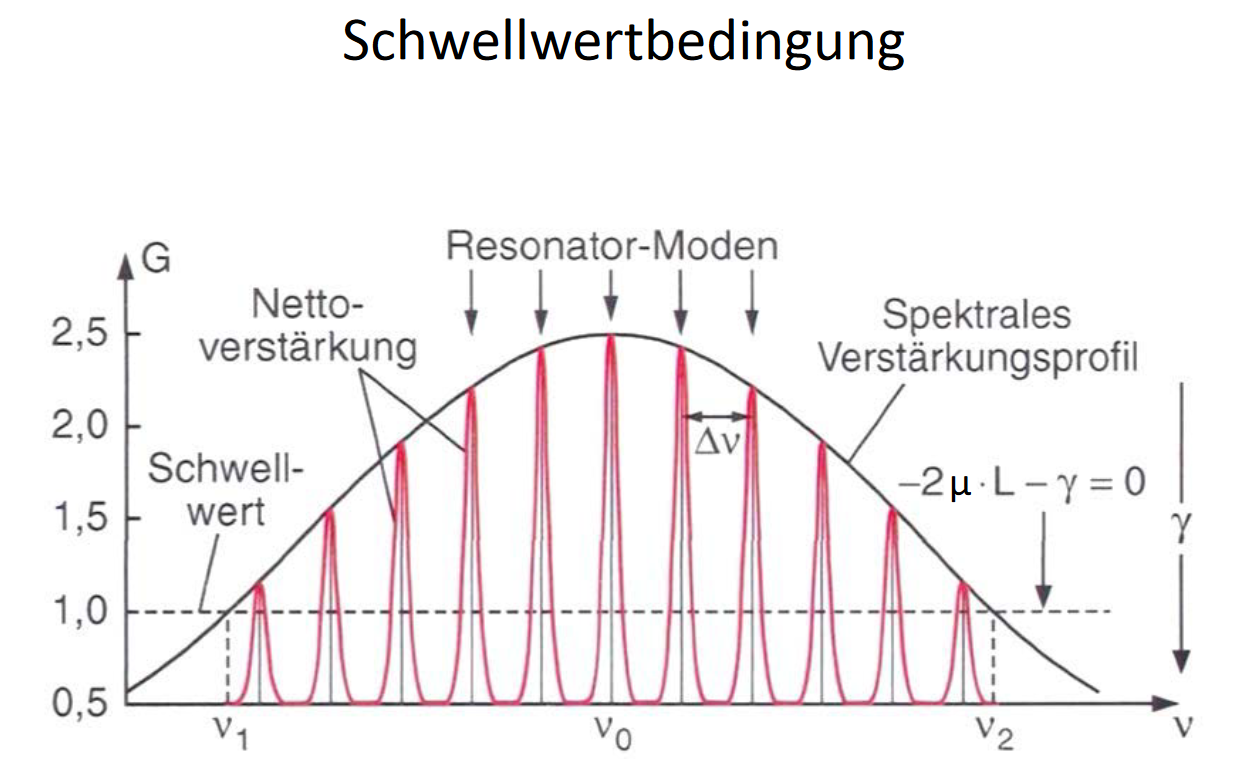
\includegraphics[width=.49\textwidth]{Schwellwertbedingung.png}
\end{figure}

\subsection{Ultra kurze Lichtpulse}
Dies funktioniert über die Nutzung des Zusammenhangs, dass ein sehr kurzes Wellenkacket ein sehr breites Frequenzspektrum hat. Über ein reflektierendes Gitter können die Wellenlängen räumlich getrennt und der
Puls damit gestreckt werden. Nach erfolgter Verstärkung wird über ein Gitter im umgekehrten Aufbau die räumliche Trennung wieder rückgängig gemacht.

\begin{figure}[H]
    \centering
    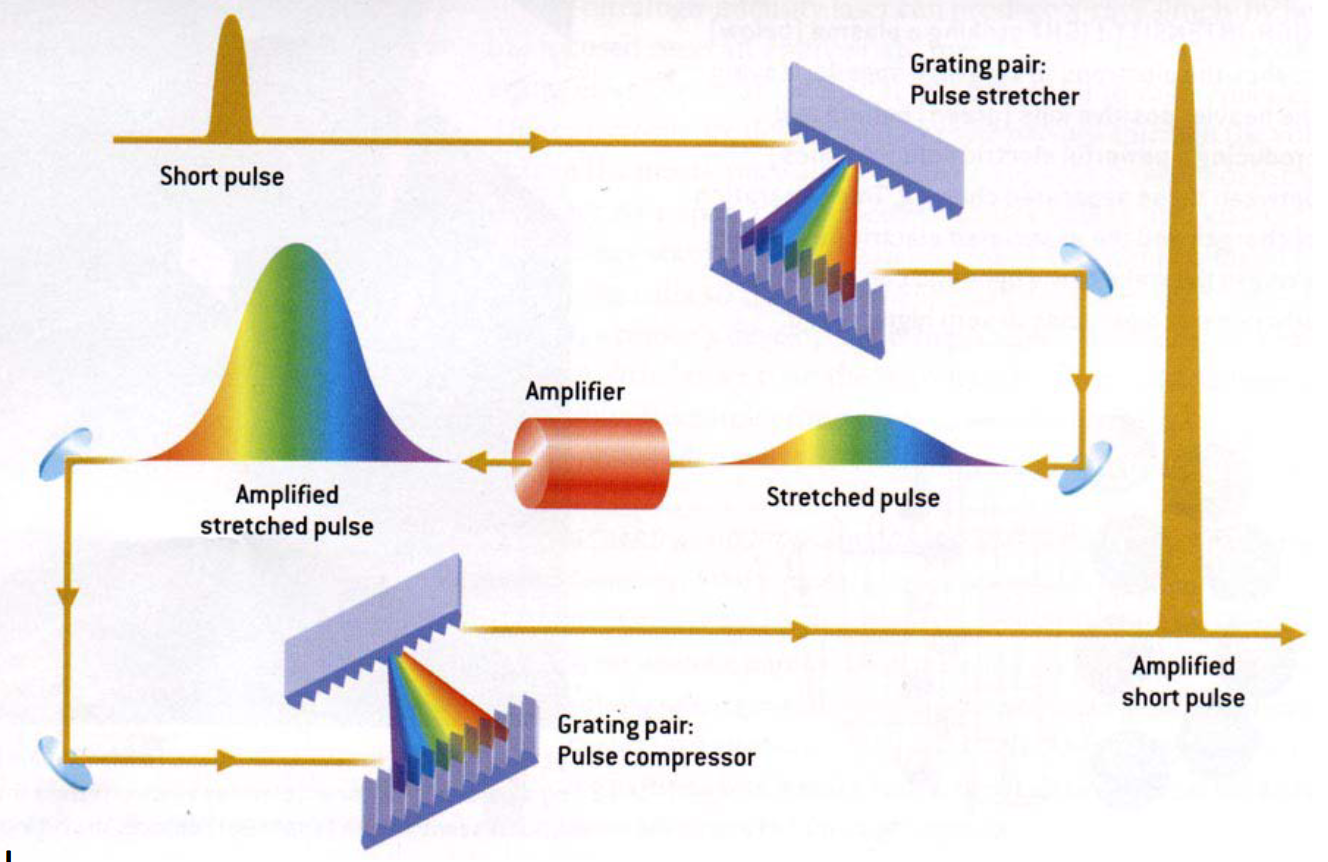
\includegraphics[width=.49\textwidth]{Kurzer_Puls.png}
\end{figure}

\subsection{Laserkühlung}
\begin{figure}[H]
    \centering
    \includegraphics[width=.49\textwidth]{Laserkühlung.png}
\end{figure}

\subsection{Frequenzkamm}
\begin{figure}[H]
    \centering
    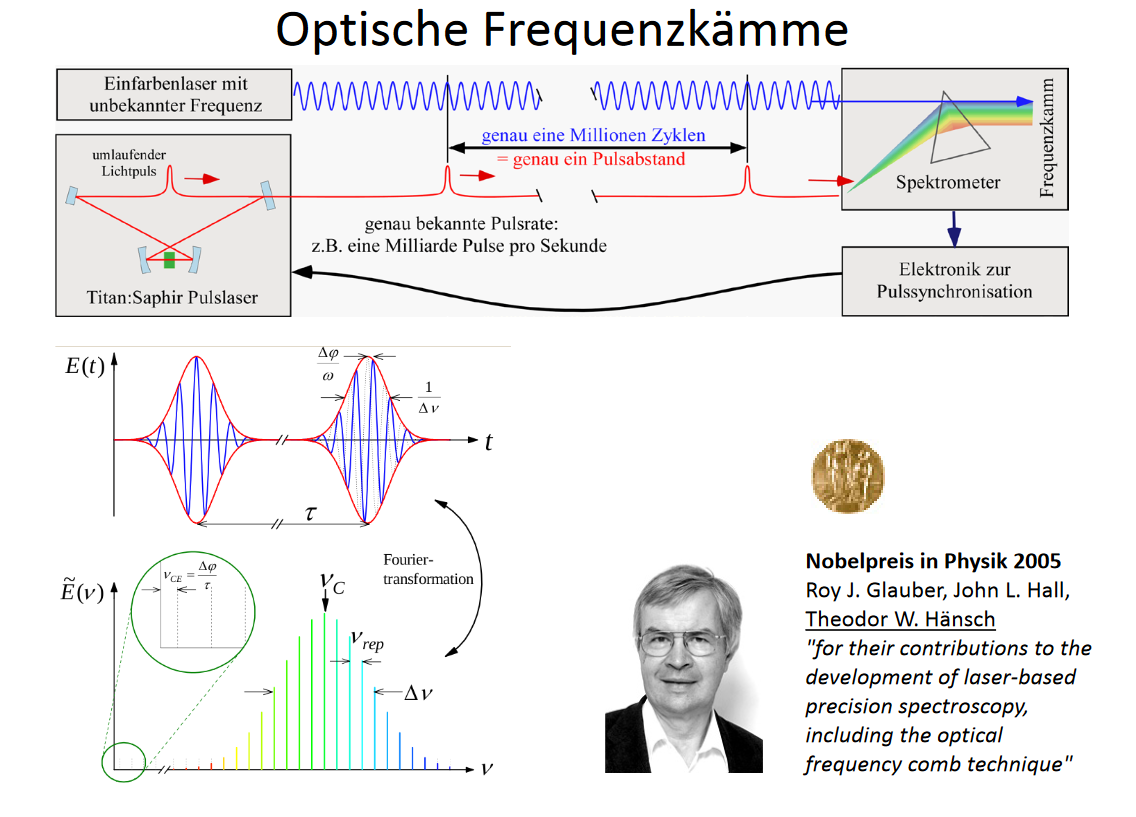
\includegraphics[width=.49\textwidth]{Frequenzkamm.png}
\end{figure}

\section{Moleküle}

\section{Experimente}

\subsection{Massenspektrometer nach Thomsons (1912)}
\begin{description}
    \item[Ziel:] Messung der atomaren Massen bzw. die relative Häufigkeit bestimmter Massen innerhalb einer Probe.
    
    \item[Aufbau:]\,

    \begin{figure}[H]
        \centering
        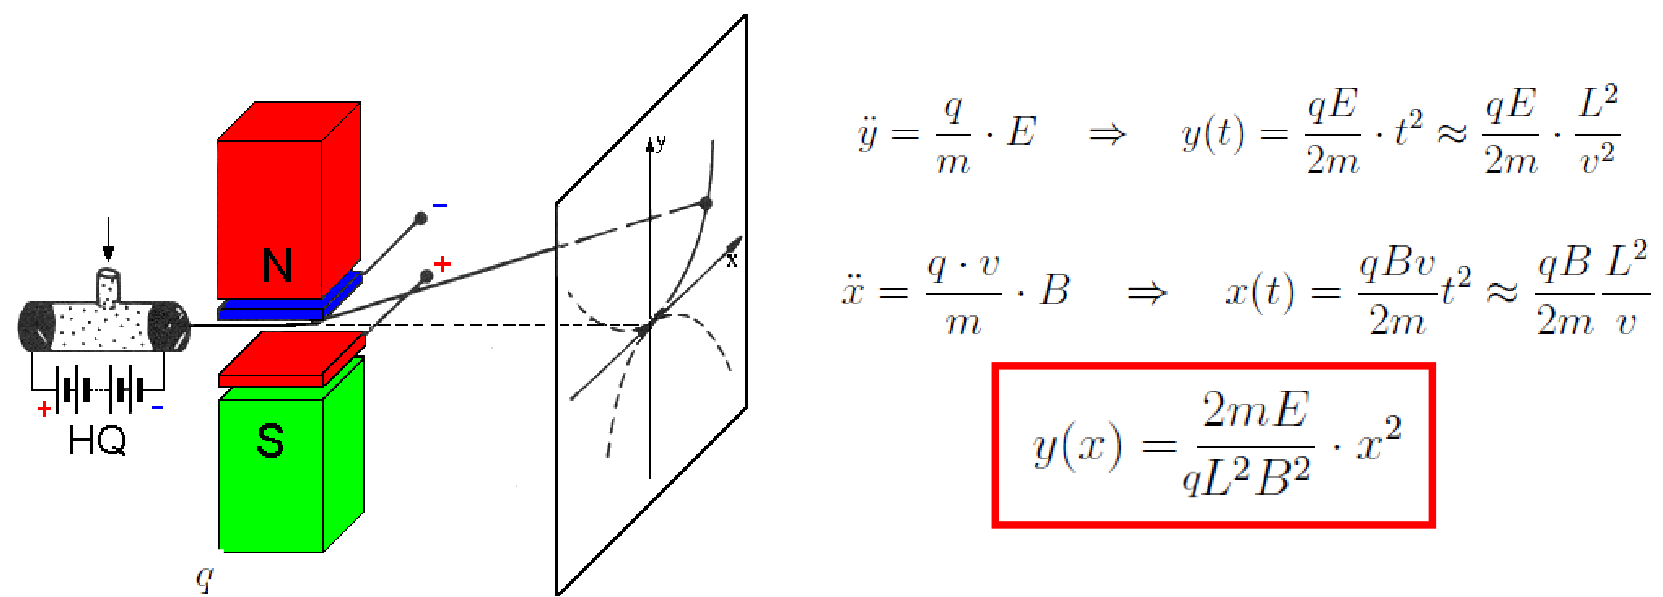
\includegraphics[width=0.49\textwidth]{massenspektrometer_nach_thomson.png}
    \end{figure}
    
    \item[Erklärung:]
    Alle Atome gleicher Masse und Ladung landen auf der gleichen Parabel, sie relative natürliche Häufgkeit einzelner Isotope kann aus der Stärke der Schwärzung im Bild eines Massenspektrometers ermittelt werden.
\end{description}

\subsection{Einstein de Haas Experiment}
\begin{description}
    \item[Ziel:] Messung des Lande Faktors \(g_s\). 
    
    \item[Aufbau:]\,
    
    \begin{figure}[H]
        \centering
        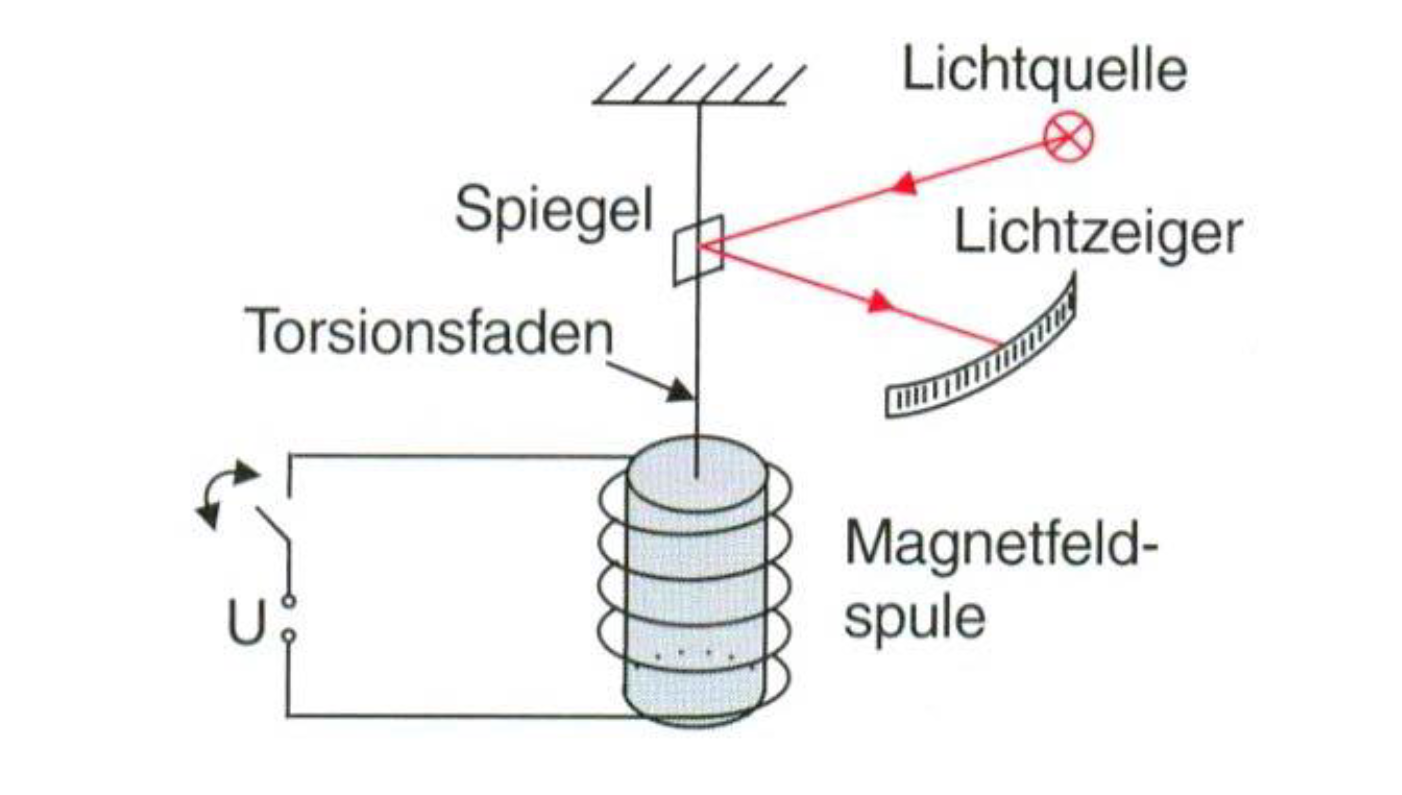
\includegraphics[width=0.49\textwidth]{Einstein_de_Haas_Experiment.pdf.png}
    \end{figure}
    
    \item[Erklärung:]
    Ein Eisenzylinder ist an einem Torsionspendel befestigt. Er wird in einer Eisenspule so stark magnetisiert, dass Sättigung erreicht wird. Dies bedeutet, dass alle Elektronenspins der $N$ freien Leitungselektronen antiparallel zur B-Feld Richtung ausgerichtet sind. Die Magnetisierung in z-Richtung ist also \(M_z = N \mu_{s,z}\). 
    Umpolung des B-Feld entspricht der Umpolung der Magnetisierung
    \begin{align*}
        \abs{\Delta M_z} &= N \abs{\Delta\mu_{s,z}} = 2N \abs{\mu_{s,z}} = N g_s \mu_B 
    \end{align*}
    Das Umklappen der Spins bedeutet aber auch eine Änderung des Drehimpulses um
    \begin{align*}
        \abs{\Delta L} &= \abs{N \Delta s_z} = N\hbar 
    \end{align*}
    Die Drehimpulsänderung entspricht einem Drehmoment, das zu einer Schwingung des Torsionspendels führt.

    Das Verhältnis von Drehimpuls und Magnetisierung
    \begin{align*}
        \frac{\Delta M}{\Delta L} &= g_s \frac{e}{2m}
    \end{align*}
    hängt nur vom Landé Faktor und Naturkonstanten ab, d.h. das Verhältnis von Drehimpuls und magnetischem
    Moment kann bestimmt werden.
\end{description}

\subsection{Penning-Falle}
\begin{description}
    \item[Ziel:] Messung des Lande Faktors \(g_s\). 
    
    \item[Aufbau:]\,
    
    \begin{figure}[H]
        \centering
        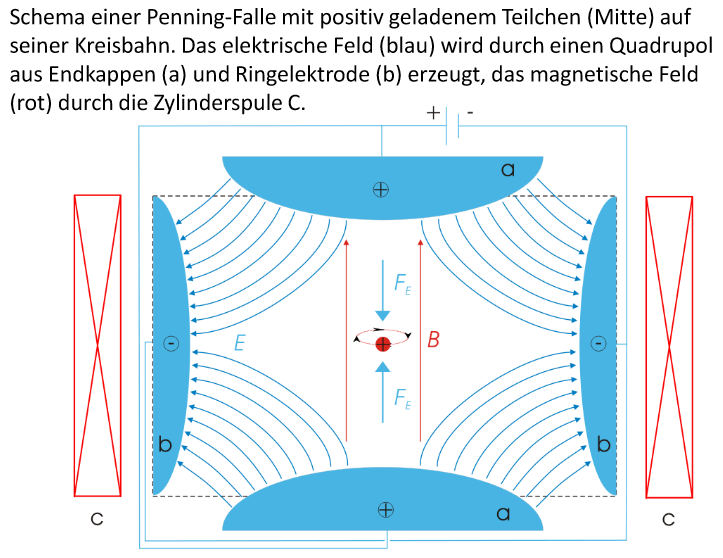
\includegraphics[width=0.49\textwidth]{Penning_Falle.png}
    \end{figure}
    
    \item[Erklärung:]
    Elektronen werden im elektrischen Quadrupolfeld und magnetischen Dipolfeld
    einer Penning Teilchenfalle eingefangen und gespeichert. Mit eingestrahlten Mikrowellen werden Spinflip Übergänge induziert.
    Aus dem Verhältnis der Zyklotron und Spinflip Frequenzen können Abweichungen von $g_s$ sehr genau bestimmt werden.
\end{description}

\subsection{Elektron-Spin Resonanz (ESR)}
\begin{description}
    \item[Ziel:] Messung des Lande Faktors in Festkörpern. Materialuntersuchungen für Proben mit ungepaarten Elektronen, oder chemische Radikalen in der Biophysik und Halbleiterphysik 
    
    \item[Aufbau:]\, Probe wird mit starkem inhomogenen Magnetfeld durchsetzt. Anschließend wird die frequenzabhängige Absorbtion von Mikrowellen vermessen.
    
    \item[Erklärung:]
    Grundlage dieses Effektes ist die Ausrichtung des magnetischen Momentes des Elektronspins in einem externen B-Feld. Hierbei definiert das B-Feld die z-Achse und die Ausrichtung entspricht einer potentiellen Energie
    \begin{align*}
        V\sub{mag} &= -\v \mu \cdot \v B = g_s \mu_b \frac{s_z}{\hbar}B = g_s \mu_B m_s B 
    \end{align*}
    Abhängig von der Spin Einstellung $m_s = \pm \frac12$ ergibt sich ein Energieunterschied zwischen den beiden Einstellungen von
    \begin{align*}
        \Delta E &= g_s \mu_B B
    \end{align*}
    Durch die frequenzabhängige Messung der Absorption von Mikrowellen in einer Probe oder
    alternativ bei einer festen Frequenz in Abhängigkeit des B-Feldes, kann sehr präzise das magnetische
    Moment bestimmt werden.
\end{description}


\subsection{Dopplerfreie Sättigungsspektroskopie}
\begin{description}
    \item[Ziel:] Messung der Hyperfeinstruktur, ohne Störung durch Dopplerverbreiterung der Linien.
    
    \item[Aufbau:]
    \begin{figure}[H]
        \centering
        \includegraphics[width=0.49\textwidth]{Dopplerfreie_Sättigungsspektroskopie.png}
    \end{figure}
    
    \item[Erklärung:]
    Grundlage dieses Effektes ist die Ausrichtung des magnetischen Momentes des Elektronspins in einem externen B-Feld. Hierbei definiert das B-Feld die z-Achse und die Ausrichtung entspricht einer potentiellen Energie
    \begin{align*}
        V\sub{mag} &= -\v \mu \cdot \v B = g_s \mu_b \frac{s_z}{\hbar}B = g_s \mu_B m_s B 
    \end{align*}
    Abhängig von der Spin Einstellung $m_s = \pm \frac12$ ergibt sich ein Energieunterschied zwischen den beiden Einstellungen von
    \begin{align*}
        \Delta E &= g_s \mu_B B
    \end{align*}
    Durch die frequenzabhängige Messung der Absorption von Mikrowellen in einer Probe oder
    alternativ bei einer festen Frequenz in Abhängigkeit des B-Feldes, kann sehr präzise das magnetische
    Moment bestimmt werden.
\end{description}


\section{Formelzeichen und ihre Bedeutung}
\begin{description}
    \item[\(r_B\):] Bohrscher Atomradius, \(r_B= \)
    \item[\(\mu_B\):] Bohrsches Magneton, \(\mu_B= \frac{e\hbar}{2m} = \begin{cases}
        9.27\E{-24}\ufrac JT\\ 5.8 \E{-5}\ufrac{eV}T
    \end{cases}\)
    \item[\(g_\ell\):] Lande Faktor für \(\ell\), \(g_\ell=1\)
    \item[\(g_s\):] Lande Faktor für \(s\), \(g_s=2\)
    \item[\(\gamma:\)] gyromagnetisches Verhältnis, \(\gamma = \frac{\absv \mu}{\absv S}\) 
    \item[\(\alpha:\)] Feinstrukturkonstante, \(\alpha = \frac{e^2}{4\pi \varepsilon_0 \hbar c}\approx \frac{1}{137}\)
    \item[\(\mu_k:\)] Kernmagneton \(\mu_k = \frac{\mu_B}{1836} = 3\E{-8} \ufrac{eV}{T}\)  
    \item[\(\Ry\):] Rybergenergie, \(\Ry = \frac{\mu Z^2 e^4}{32\pi^2 \hbar^2 \epsilon_0^2} = 13.6\u{eV}\)  
    \item[\(R_\inf\):] Rybergwellenlänge, \(R_\inf = \frac{\Ry}{hc}\)  
\end{description}

\end{document}